\documentclass{article}
\usepackage[utf8]{inputenc}
\usepackage{geometry}
\usepackage{listings}
\usepackage{xcolor}
\usepackage{hyperref}
\usepackage{graphicx}
\usepackage{tikz}
\usepackage{amsmath}
\usepackage{booktabs}
\usepackage{longtable}

\geometry{a4paper, margin=1in}

% Colors
\definecolor{codegreen}{rgb}{0,0.6,0}
\definecolor{codegray}{rgb}{0.5,0.5,0.5}
\definecolor{codepurple}{rgb}{0.58,0,0.82}
\definecolor{backcolour}{rgb}{0.95,0.95,0.92}
\definecolor{cosmosbg}{rgb}{0.04,0.06,0.12}
\definecolor{cosmosaccent}{rgb}{0.53,0.67,1.0}

% Code styling
\lstdefinestyle{mystyle}{
    backgroundcolor=\color{backcolour},
    commentstyle=\color{codegreen},
    keywordstyle=\color{blue},
    numberstyle=\tiny\color{codegray},
    stringstyle=\color{codepurple},
    basicstyle=\ttfamily\small,
    breaklines=true,
    frame=single,
    numbers=left,
    tabsize=4
}

\lstset{style=mystyle}

% Hyperlinks
\hypersetup{
    colorlinks=true,
    linkcolor=cosmosaccent,
    filecolor=magenta,
    urlcolor=cyan,
}

\title{\textbf{Cosmos Simulation}\\\large API Documentation v2.0}
\author{Cosmos Simulation Team}
\date{\today}

\begin{document}

\maketitle
\thispagestyle{empty}

\vspace{2cm}

\begin{center}
\includegraphics[width=0.5\textwidth]{Resources/Assets/images/logo.png}
\end{center}

\vspace{2cm}

\begin{center}
\textbf{A Comprehensive Solar System Simulation}\\\large
Three.js-based 3D visualization with Keplerian orbital mechanics
\end{center}

\vspace{3cm}

\begin{table}[h]
\centering
\begin{tabular}{ll}
\textbf{Version} & 2.0.0 \\
\textbf{Last Updated} & \today \\
\textbf{License} & MIT \\
\textbf{Repository} & github.com/cosmos-simulation
\end{tabular}
\end{table}

\newpage
\tableofcontents
\newpage

% ==============================================================================
% SECTION: ASTRONOMICAL DATA
% ==============================================================================
\section{AstronomicalData API Reference}
\label{sec:astronomicaldata}

Provides comprehensive solar system celestial body data including planets, moons, comets, and meteor showers. Data is sourced from NASA/JPL databases.

\subsection{Overview}

\begin{figure}[htbp]
\centering
\begin{tikzpicture}[scale=0.8]
    % Sun
    \draw[fill=yellow] (0,0) circle (1cm);
    \node at (0,-1.5) {Sun};
    
    % Planets orbits
    \draw[dotted] (0,0) circle (2.5cm);
    \draw[dotted] (0,0) circle (3.5cm);
    \draw[dotted] (0,0) circle (5cm);
    \draw[dotted] (0,0) circle (8cm);
    \draw[dotted] (0,0) circle (12cm);
    
    % Planets
    \draw[fill=gray] (2.5,0) circle (0.2cm) node[below] {Mercury};
    \draw[fill=orange] (3.5,0) circle (0.25cm) node[below] {Venus};
    \draw[fill=blue] (5,0) circle (0.3cm) node[below] {Earth};
    \draw[fill=red] (6.5,0) circle (0.25cm) node[below] {Mars};
    \draw[fill=brown] (8,0) circle (0.8cm) node[below] {Jupiter};
    \draw[fill=gold] (12,0) circle (0.7cm) node[below] {Saturn};
\end{tikzpicture}
\caption{Solar System Overview}
\label{fig:solarsystem}
\end{figure}

\subsection{Constants}

\begin{longtable}{|l|l|p{6cm}|}
\hline
\textbf{Constant} & \textbf{Value} & \textbf{Description} \\
\hline
AU & 149597870700 & Astronomical Unit in meters (Earth-Sun distance) \\
\hline
DAY & 86400 & Seconds per day \\
\hline
DEG2RAD & $\pi / 180$ & Degrees to radians conversion factor \\
\hline
RAD2DEG & $180 / \pi$ & Radians to degrees conversion factor \\
\hline
J2000 & Jan 1, 2000 12:00:00 UTC & J2000 epoch reference date \\
\hline
\end{longtable}

\subsection{Celestial Body Structure}

\begin{lstlisting}
{
    name: "BodyName",
    type: "planet|moon|comet|meteor|star",
    parent: "ParentBodyName",
    a: 1.524,              // Semi-major axis (AU for planets)
    e: 0.093,              // Eccentricity (0-1)
    i: 7.0,                // Inclination (degrees)
    radius: 3390000,       // Mean radius in meters
    mass: 6.39e+23,        // Mass in kg
    period: 687,           // Orbital period in days
    rotation: 24.6,        // Rotation period in hours
    tilt: 25.2,            // Axial tilt in degrees
    color: 0xC1440E,       // Hex color for visualization
    moons: ["Moon1", "Moon2"]
}
\end{lstlisting}

\subsection{Methods}

\subsection*{getAllBodies()}

Returns an object containing all celestial bodies indexed by name.

\subsection*{getMoonsForPlanet(planetName)}

Returns an array of moon objects for the specified planet.

% ==============================================================================
% SECTION: PHYSICS ENGINE
% ==============================================================================
\section{PhysicsEngine API Reference}
\label{sec:physicsengine}

Implements ultra-accurate orbital mechanics using Keplerian physics with J2000 epoch reference.

\subsection{Kepler's Equation Solver}

\begin{figure}[htbp]
\centering
\begin{tikzpicture}[node distance=2cm]
    \node (start) [rectangle, draw] {Start: Mean Anomaly M, Eccentricity e};
    \node (calc) [rectangle, draw, below of=start] {Calculate initial guess $E_0$};
    \node (iterate) [rectangle, draw, below of=calc] {Newton-Raphson iteration};
    \node (check) [diamond, draw, below of=iterate] {Converged?};
    \node (output) [rectangle, draw, right of=check, xshift=3cm] {Output: Eccentric Anomaly E};
    \node (loop) [rectangle, draw, below of=check, yshift=-2cm] {Update E, repeat};

    \draw[->] (start) -- (calc);
    \draw[->] (calc) -- (iterate);
    \draw[->] (iterate) -- (check);
    \draw[->] (check) -- node[above] {Yes} (output);
    \draw[->] (check) -- node[right] {No} (loop);
    \draw[->] (loop) -- (iterate);
\end{tikzpicture}
\caption{Kepler's Equation Solver Flow}
\label{fig:keplerflow}
\end{figure}

\subsection{Methods}

\subsection*{deg2rad(degrees)}

Converts degrees to radians.

\subsection*{rad2deg(radians)}

Converts radians to degrees.

\subsection*{solveKepler(M, e, tolerance)}

Solves Kepler's equation using Newton-Raphson iteration.

\begin{equation}
M = E - e \cdot \sin(E)
\end{equation}

Where:
\begin{itemize}
    \item M = Mean anomaly
    \item E = Eccentric anomaly
    \item e = Eccentricity
\end{itemize}

\subsection*{calculatePosition(elements, time)}

Calculates 3D position from orbital elements at a given time.

\subsection*{calculatePeriod(a)}

Calculates orbital period from semi-major axis using Kepler's 3rd law.

\begin{equation}
P^2 = a^3
\end{equation}

% ==============================================================================
% SECTION: TIME SYSTEM
% ==============================================================================
\section{TimeSystem API Reference}
\label{sec:timesystem}

Manages simulation time, date calculations, time scales, and calendar conversions.

\subsection{Time Update Flow}

\begin{figure}[htbp]
\centering
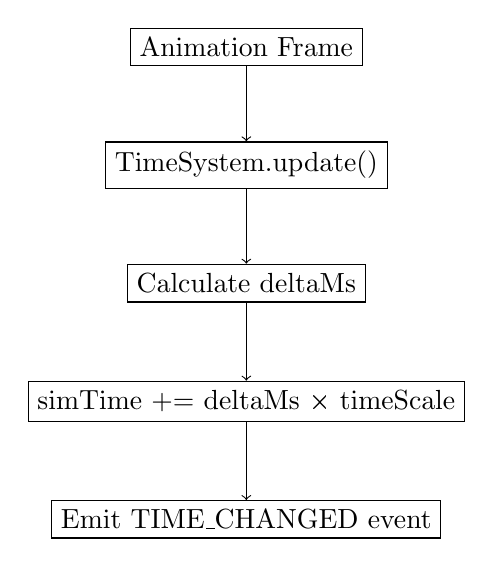
\begin{tikzpicture}[node distance=1.5cm]
    \node (frame) [rectangle, draw] {Animation Frame};
    \node (update) [rectangle, draw, below of=frame] {TimeSystem.update()};
    \node (delta) [rectangle, draw, below of=update] {Calculate deltaMs};
    \node (apply) [rectangle, draw, below of=delta] {simTime += deltaMs × timeScale};
    \node (notify) [rectangle, draw, below of=apply] {Emit TIME\_CHANGED event};
    
    \draw[->] (frame) -- (update);
    \draw[->] (update) -- (delta);
    \draw[->] (delta) -- (apply);
    \draw[->] (apply) -- (notify);
\end{tikzpicture}
\caption{Time Update Sequence}
\label{fig:timeflow}
\end{figure}

\subsection{Time Scale Presets}

\begin{table}[h]
\centering
\begin{tabular}{|l|l|}
\hline
\textbf{Preset Name} & \textbf{Value} \\
\hline
paused & 0 \\
realtime & 1 \\
1min/sec & 60 \\
1hour/sec & 3600 \\
1day/sec & 86400 \\
1week/sec & 604800 \\
1year/sec & 31536000 \\
10years/sec & 315360000 \\
\hline
\end{tabular}
\caption{Time Scale Presets}
\end{table}

% ==============================================================================
% SECTION: WEBGL RENDERER
% ==============================================================================
\section{WebGLRenderer API Reference}
\label{sec:webglrenderer}

Three.js-based 3D visualization engine for rendering the solar system.

\subsection{Scene Graph Structure}

\begin{figure}[htbp]
\centering
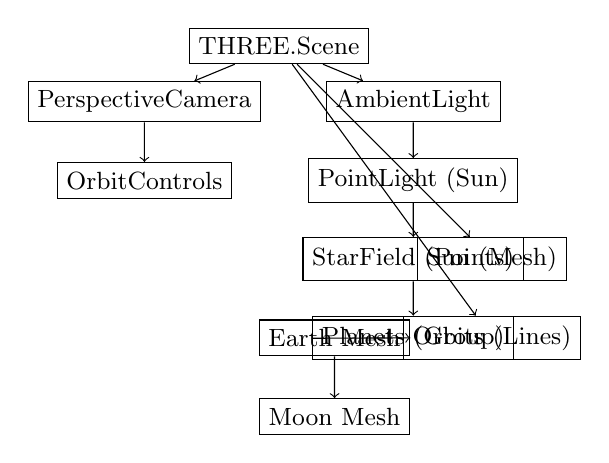
\begin{tikzpicture}[scale=0.7, every node/.style={font=\small}]
    \node (scene) [rectangle, draw] {THREE.Scene};
    \node (camera) [rectangle, draw, below left of=scene, xshift=-1cm] {PerspectiveCamera};
    \node (controls) [rectangle, draw, below of=camera] {OrbitControls};
    \node (ambient) [rectangle, draw, below right of=scene, xshift=1cm] {AmbientLight};
    \node (point) [rectangle, draw, below of=ambient] {PointLight (Sun)};
    \node (stars) [rectangle, draw, below of=point] {StarField (Points)};
    \node (sun) [rectangle, draw, right of=stars] {Sun (Mesh)};
    \node (planets) [rectangle, draw, below of=stars] {Planets (Group)};
    \node (earth) [rectangle, draw, left of=planets] {Earth Mesh};
    \node (moon) [rectangle, draw, below of=earth] {Moon Mesh};
    \node (orbits) [rectangle, draw, right of=planets] {Orbits (Lines)};

    \draw[->] (scene) -- (camera);
    \draw[->] (camera) -- (controls);
    \draw[->] (scene) -- (ambient);
    \draw[->] (ambient) -- (point);
    \draw[->] (point) -- (stars);
    \draw[->] (stars) -- (planets);
    \draw[->] (planets) -- (earth);
    \draw[->] (earth) -- (moon);
    \draw[->] (scene) -- (sun);
    \draw[->] (scene) -- (orbits);
\end{tikzpicture}
\caption{Three.js Scene Graph Structure}
\label{fig:scenegraph}
\end{figure}

% ==============================================================================
% SECTION: INTEGRATION
% ==============================================================================
\section{Integration API Reference}
\label{sec:integration}

Documentation for how the Cosmos Simulation engine components interact.

\subsection{System Architecture}

\begin{figure}[htbp]
\centering
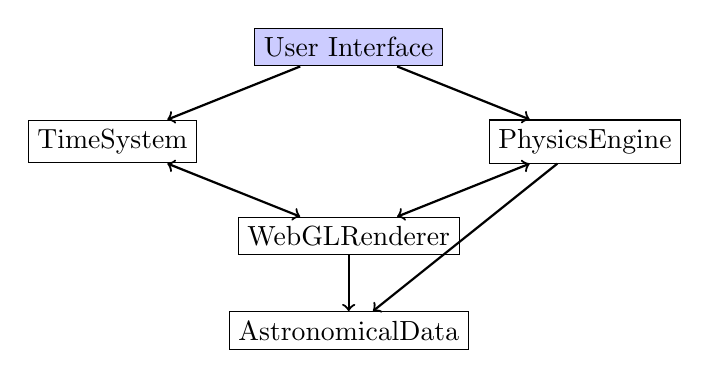
\begin{tikzpicture}[node distance=1.2cm]
    % User Interface
    \node (ui) [rectangle, draw, fill=blue!20] {User Interface};
    
    % Engines
    \node (time) [rectangle, draw, below of=ui, xshift=-3cm] {TimeSystem};
    \node (physics) [rectangle, draw, below of=ui, xshift=3cm] {PhysicsEngine};
    
    % Renderer
    \node (renderer) [rectangle, draw, below of=time, xshift=3cm] {WebGLRenderer};
    
    % Data
    \node (data) [rectangle, draw, below of=renderer] {AstronomicalData};
    
    % Arrows
    \draw[->, thick] (ui) -- (time);
    \draw[->, thick] (ui) -- (physics);
    \draw[<->, thick] (time) -- (renderer);
    \draw[<->, thick] (physics) -- (renderer);
    \draw[->, thick] (physics) -- (data);
    \draw[->, thick] (renderer) -- (data);
\end{tikzpicture}
\caption{Engine Integration Diagram}
\label{fig:integration}
\end{figure}

% ==============================================================================
% SECTION: ARCHITECTURE
% ==============================================================================
\section{Architecture API Reference}
\label{sec:architecture}

System architecture and module structure.

\subsection{Layer Architecture}

\begin{figure}[htbp]
\centering
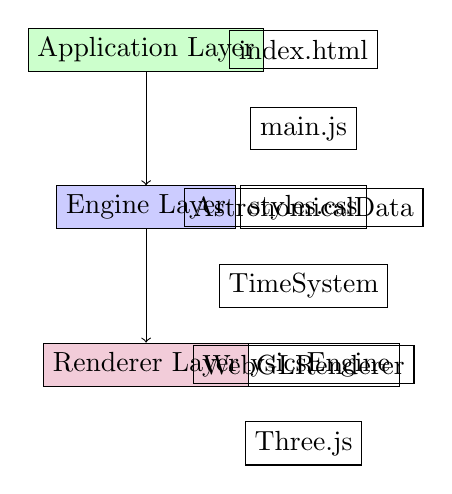
\begin{tikzpicture}[node distance=1cm]
    % Application Layer
    \node (app) [rectangle, draw, fill=green!20] {Application Layer};
    \node (html) [rectangle, draw, right of=app, xshift=1cm] {index.html};
    \node (js) [rectangle, draw, below of=html] {main.js};
    \node (css) [rectangle, draw, below of=js] {styles.css};
    
    % Engine Layer
    \node (engine) [rectangle, draw, below of=app, yshift=-1cm, fill=blue!20] {Engine Layer};
    \node (astro) [rectangle, draw, right of=engine, xshift=1cm] {AstronomicalData};
    \node (timeeng) [rectangle, draw, below of=astro] {TimeSystem};
    \node (physicseng) [rectangle, draw, below of=timeeng] {PhysicsEngine};
    
    % Renderer Layer
    \node (render) [rectangle, draw, below of=engine, yshift=-1cm, fill=purple!20] {Renderer Layer};
    \node (webgl) [rectangle, draw, right of=render, xshift=1cm] {WebGLRenderer};
    \node (three) [rectangle, draw, below of=webgl] {Three.js};
    
    % Arrows
    \draw[->] (app) -- (engine);
    \draw[->] (engine) -- (render);
\end{tikzpicture}
\caption{Layer Architecture}
\label{fig:layers}
\end{figure}

% ==============================================================================
% SECTION: CONFIGURATION
% ==============================================================================
\section{Configuration API Reference}
\label{sec:configuration}

Complete reference for all configuration options.

\subsection{WebGLRenderer Settings}

\begin{longtable}{|l|l|l|}
\hline
\textbf{Setting} & \textbf{Type} & \textbf{Default} \\
\hline
showOrbits & boolean & false \\
\hline
showLabels & boolean & false \\
\hline
showAsteroids & boolean & false \\
\hline
showMoons & boolean & true \\
\hline
scalePlanets & number & 0.0001 \\
\hline
orbitOpacity & number & 0.3 \\
\hline
starFieldDensity & number & 100 \\
\hline
asteroidCount & number & 50 \\
\hline
minDistance & number & 1 \\
\hline
maxDistance & number & 10000 \\
\hline
\end{longtable}

% ==============================================================================
% SECTION: COMPONENTS
% ==============================================================================
\section{Components API Reference}
\label{sec:components}

UI component documentation.

\subsection{UI Layout}

\begin{figure}[htbp]
\centering
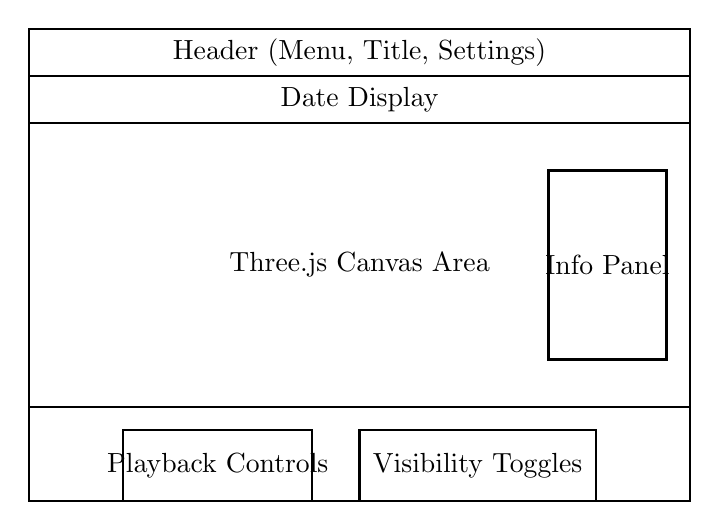
\begin{tikzpicture}[scale=0.6]
    % Main container
    \draw[thick] (0,0) rectangle (14,10);
    
    % Header
    \draw[thick] (0,9) rectangle (14,10);
    \node at (7,9.5) {Header (Menu, Title, Settings)};
    
    % Date display
    \draw[thick] (0,8) rectangle (14,9);
    \node at (7,8.5) {Date Display};
    
    % Canvas
    \draw[thick] (0,2) rectangle (14,8);
    \node at (7,5) {Three.js Canvas Area};
    
    % Info panel
    \draw[thick] (11,3) rectangle (13.5,7);
    \node at (12.25,5) {Info Panel};
    
    % Time controls
    \draw[thick] (2,0) rectangle (6,1.5);
    \node at (4,0.75) {Playback Controls};
    
    % Toggles
    \draw[thick] (7,0) rectangle (12,1.5);
    \node at (9.5,0.75) {Visibility Toggles};
\end{tikzpicture}
\caption{UI Component Layout}
\label{fig:uilayout}
\end{figure}

% ==============================================================================
% SECTION: EVENTS
% ==============================================================================
\section{Events API Reference}
\label{sec:events}

Event system documentation.

\subsection{Event Flow}

\begin{figure}[htbp]
\centering
\begin{tikzpicture}[node distance=2cm]
    % Source
    \node (source) [rectangle, draw, fill=red!20] {Source Component};
    
    % Event Bus
    \node (bus) [ellipse, draw, fill=yellow!20, right of=source, xshift=3cm] {Event Bus};
    
    % Handlers
    \node (handler1) [rectangle, draw, below of=bus] {Handler 1};
    \node (handler2) [rectangle, draw, right of=handler1, xshift=2cm] {Handler 2};
    \node (handler3) [rectangle, draw, left of=handler1, xshift=-2cm] {Handler 3};
    
    % Arrows
    \draw[->, thick] (source) -- (bus) node[midway, above] {emit()};
    \draw[->, thick] (bus) -- (handler1) node[midway, left] {on()};
    \draw[->, thick] (bus) -- (handler2);
    \draw[->, thick] (bus) -- (handler3);
\end{tikzpicture}
\caption{Event Flow Diagram}
\label{fig:eventflow}
\end{figure}

\subsection{Event Types}

\begin{table}[h]
\centering
\begin{tabular}{|l|l|}
\hline
\textbf{Event} & \textbf{Description} \\
\hline
cosmos:time-changed & Fired when simulation time changes \\
\hline
cosmos:body-selected & Fired when a celestial body is selected \\
\hline
cosmos:body-deselected & Fired when selection is cleared \\
\hline
cosmos:play-state-changed & Fired when play/pause state changes \\
\hline
cosmos:window-resized & Fired when window is resized \\
\hline
cosmos:physics-error & Fired when physics calculation fails \\
\hline
\end{tabular}
\end{table}

% ==============================================================================
% APPENDIX
% ==============================================================================
\section{Appendix}

\subsection{Orbital Element Definitions}

\begin{table}[h]
\centering
\begin{tabular}{|l|l|p{7cm}|}
\hline
\textbf{Symbol} & \textbf{Name} & \textbf{Description} \\
\hline
a & Semi-major axis & Average distance from parent body \\
\hline
e & Eccentricity & Shape of orbit (0 = circle, 1 = parabola) \\
\hline
i & Inclination & Tilt of orbital plane (degrees) \\
\hline
w & Longitude of perihelion & Position of closest approach \\
\hline
node & Longitude of ascending node & Where orbit crosses reference plane \\
\hline
L & Mean longitude & Average angular position \\
\hline
\end{tabular}
\end{table}

\subsection{Data Sources}

\begin{itemize}
    \item Open Solar System API (api.le-systeme-solaire.net)
    \item NASA Planetary Fact Sheet
    \item JPL Small-Body Database
\end{itemize}

\subsection{License}

This documentation is part of the Cosmos Simulation project, licensed under the MIT License.

\end{document}

